\section{Database model}\label{sec:database-model}
There is a database model to store data in Dronetag backend.
The database model consists followings entities:
\begin{itemize}
    \item User,
    \item Aircraft,
    \item Device,
    \item Flight,
    \item Telemetry measurement,
    \item Organization,
    \item Fleet,
    \item Aircraft vendor,
    \item Aircraft model,
    \item Airspace zone,
    \item User preference and
    \item Organization preference.
\end{itemize}
A detailed diagram with relationships between entities is in the ERD Diagram of infrastructure in the picture~\ref{fig:erd-diagram}.

\subsection{User}\label{subsec:user}
This entity represents a user who signs up and logs in to the application.
It consists of user credentials and identification information.

All attributes are described like this:
\begin{itemize}
    \item id - represents the unique object identificator,
    \item email - represents the e-mail that a user will be log in to the system and receive notifications,
    \item full\_name - represents optional full name of the user,
    \item password\_hash - represents a hashed password,
    \item phone\_number - represents a phone number that a user will be able to contact in case of emergency,
    \item deleted - represents a boolean flag that will be set if a user want to delete his account,
    \item date\_created - represents a date of registration,
    \item date\_modified - represents a date of modification,
    \item last\_login - represents a date of last log in,
    \item active - represents a boolean flag if a user is active and
    \item country - represents a country where a user is used to be flying.
\end{itemize}

\subsection{Aircraft}\label{subsec:aircraft}
This entity represents an aircraft that is connect with a Dronetag device.
... %TODO

All attributes are described like this:
\begin{itemize}
    \item id - represents the unique object identificator,
    \item name - represents an aircraft name for easier recognition in My aircraft list,
    \item uas\_operator\_id - represents a unique code identifying a pilot who registered this aircraft,
    \item weight - represents a weight of the aircraft,
    \item date\_created - represents a date when an aircraft was added,
    \item data\_modified - represents a date when an aircraft was changed,
    \item deleted - represents a boolean flag if an aircraft was deleted.
\end{itemize}

\subsection{Device}\label{subsec:device}
This entity represents a physical device that sends live information to the Dronetag platform.
... %TODO

All attributes are described like this:
\begin{itemize}
    \item id - represents the unique object identificator,
    \item serial\_number - represents a serial number of a device,
    \item name - represents a device name for easier recognition in My aircraft list,
    \item type - represents
    \item comm\_id - represents a communication identificator via CoAP,
    \item date\_created - represents a date when a device was added,
    \item date\_modified - represents a date when a device was changed,
    \item last\_battery - represents a last battery value in Volts,
    \item last\_rsrp - represents a RSRP (Reference Signal Receive Power) value and
    \item last\_message - represents a received CoAP message.
\end{itemize}

\subsection{Flight}\label{subsec:flight}
This entity represents it represents a flight that a user has created.
... %TODO

All attributes are described like this:
\begin{itemize}
    \item id - represents the unique object identificator,
    \item date\_planned\_start - represents a start date of planned flight,
    \item date\_planned\_finish - represents a finish data of planned flight,
    \item date\_started - represents a real start date of flight,
    \item date\_finished - represents a real finish date of flight,
    \item status - represents a flight status - values can be "planned", "current", "finished" and "canceled",
    \item distance - represents a distance of flight,
    \item duration - represents a duration of flight,
    \item region\_geojson - represents a reservation region in GeoJSON format \cite{geoJson},
    \item max\_flight\_altitude - represents a maximum flight altitude,
    \item takeoff\_latitude - represents a latitude of take off position,
    \item takeoff\_longitude - represents a longitude of take off position,
    \item takeoff\_geo\_alt - represents a geological altitude of take off position,
    \item takeoff\_pressure - represents a take off pressure,
    \item public - represents a boolean flag if a flight is public (visible for everyone),
    \item date\_created - represents a date when a flight was added,
    \item date\_modified - represents a date when a flight was changed and
    \item deleted - represents a boolean flag if a flight was deleted.
\end{itemize}

\subsection{Telemetry measurement}\label{subsec:telemetry-measurement}
This entity represents a telemetry measurement that the system receives and thanks that we are able to draw a flight trajectory.

All attributes are described like this:
\begin{itemize}
    \item time\_received - represents the unique object identificator,
    \item time - represents a date with time of measurement,
    \item latitude - represents a measured latitude of a flying drone,
    \item longitude - represents a measured longitude of a flying drone,
    \item altitude - represents a measured altitude of a flying drone,
    \item geo\_altitude - represents a measured geological altitude of a flying drone,
    \item velocity\_x - represents a measured velocity in X axis,
    \item velocity\_y - represents a measured velocity in Y axis,
    \item velocity\_z - represents a measured velocity in Z axis and
    \item gnss\_accuracy - represents a (GNSS) Global Navigation Satellite System accuracy.
\end{itemize}

\subsection{Organization}\label{subsec:organization}
This entity represents an Organization for maintenance of fleet management.

All attributes are described like this:
\begin{itemize}
    \item id - represents the unique object identificator,
    \item name - represents a name of an organization,
    \item description - represents a text descripton of an organization
    \item date\_created - represents a date when an organization was added,
    \item date\_modified - represents a date when an organization was changed and
    \item deleted - represents a boolean flag if an organization was deleted.
\end{itemize}

\subsection{Fleet}\label{subsec:fleet}
This entity represents an organization's fleet management properties.

All attributes are described like this:
\begin{itemize}
    \item id - represents the unique object identificator,
    \item name - represents a name of a fleet,
    \item color - represents a shown color of a fleet,
    \item deleted - represents a boolean flag if a fleet was deleted,
    \item date\_created - represents a date when a fleet was added and
    \item date\_modified - represents a date when a fleet was changed.
\end{itemize}

\subsection{Aircraft vendor}\label{subsec:aircraft-vendor}
This entity represents an aircraft vendor who manufactures drones.

All attributes are described like this:
\begin{itemize}
    \item id - represents the unique object identificator,
    \item name - represents a vendor name.
\end{itemize}

\subsection{Aircraft model}\label{subsec:aircraft-model}
This entity represents an aircraft model that belongs to a vendor.
... %TODO

All attributes are described like this:
\begin{itemize}
    \item id - represents the unique object identificator,
    \item name - represents a model name,
    \item weight - represents a weight of a model and
    \item vendor\_id - represents a relationship to a Vendor.
\end{itemize}

\subsection{Airspace zone}\label{subsec:airspace-zone}
This entity represents an airspace zone

All attributes are described like this:
\begin{itemize}
    \item id - represents the unique object identificator,
    \item name - represents a name of a zone,
    \item country - represents a country where a zone belongs,
    \item region\_geojson - represents a region in GeoJSON format \cite{geoJson},
    \item date\_created - represents a date when a fleet was added and
    \item date\_modified - represents a date when a fleet was changed.
\end{itemize}

\subsection{User preference}\label{subsec:user-preference}
This entity represents a user preference that is needed to store and share among various clients.

All attributes are described like this:
\begin{itemize}
    \item property - represents an identificator of property,
    \item value - represents a preference value and
    \item date\_modified - represents a date when a preference was changed.
\end{itemize}

\subsection{Organization preference}\label{subsec:organization-preference}
This entity represents an organization preference that is neede to store and share among various clients.

All attributes are described like this:
\begin{itemize}
    \item property - represents the identificator of property,
    \item value - represents a preference value and
    \item date\_modified - represents a date when a preference was changed.
\end{itemize}

\begin{figure}
    \centering
    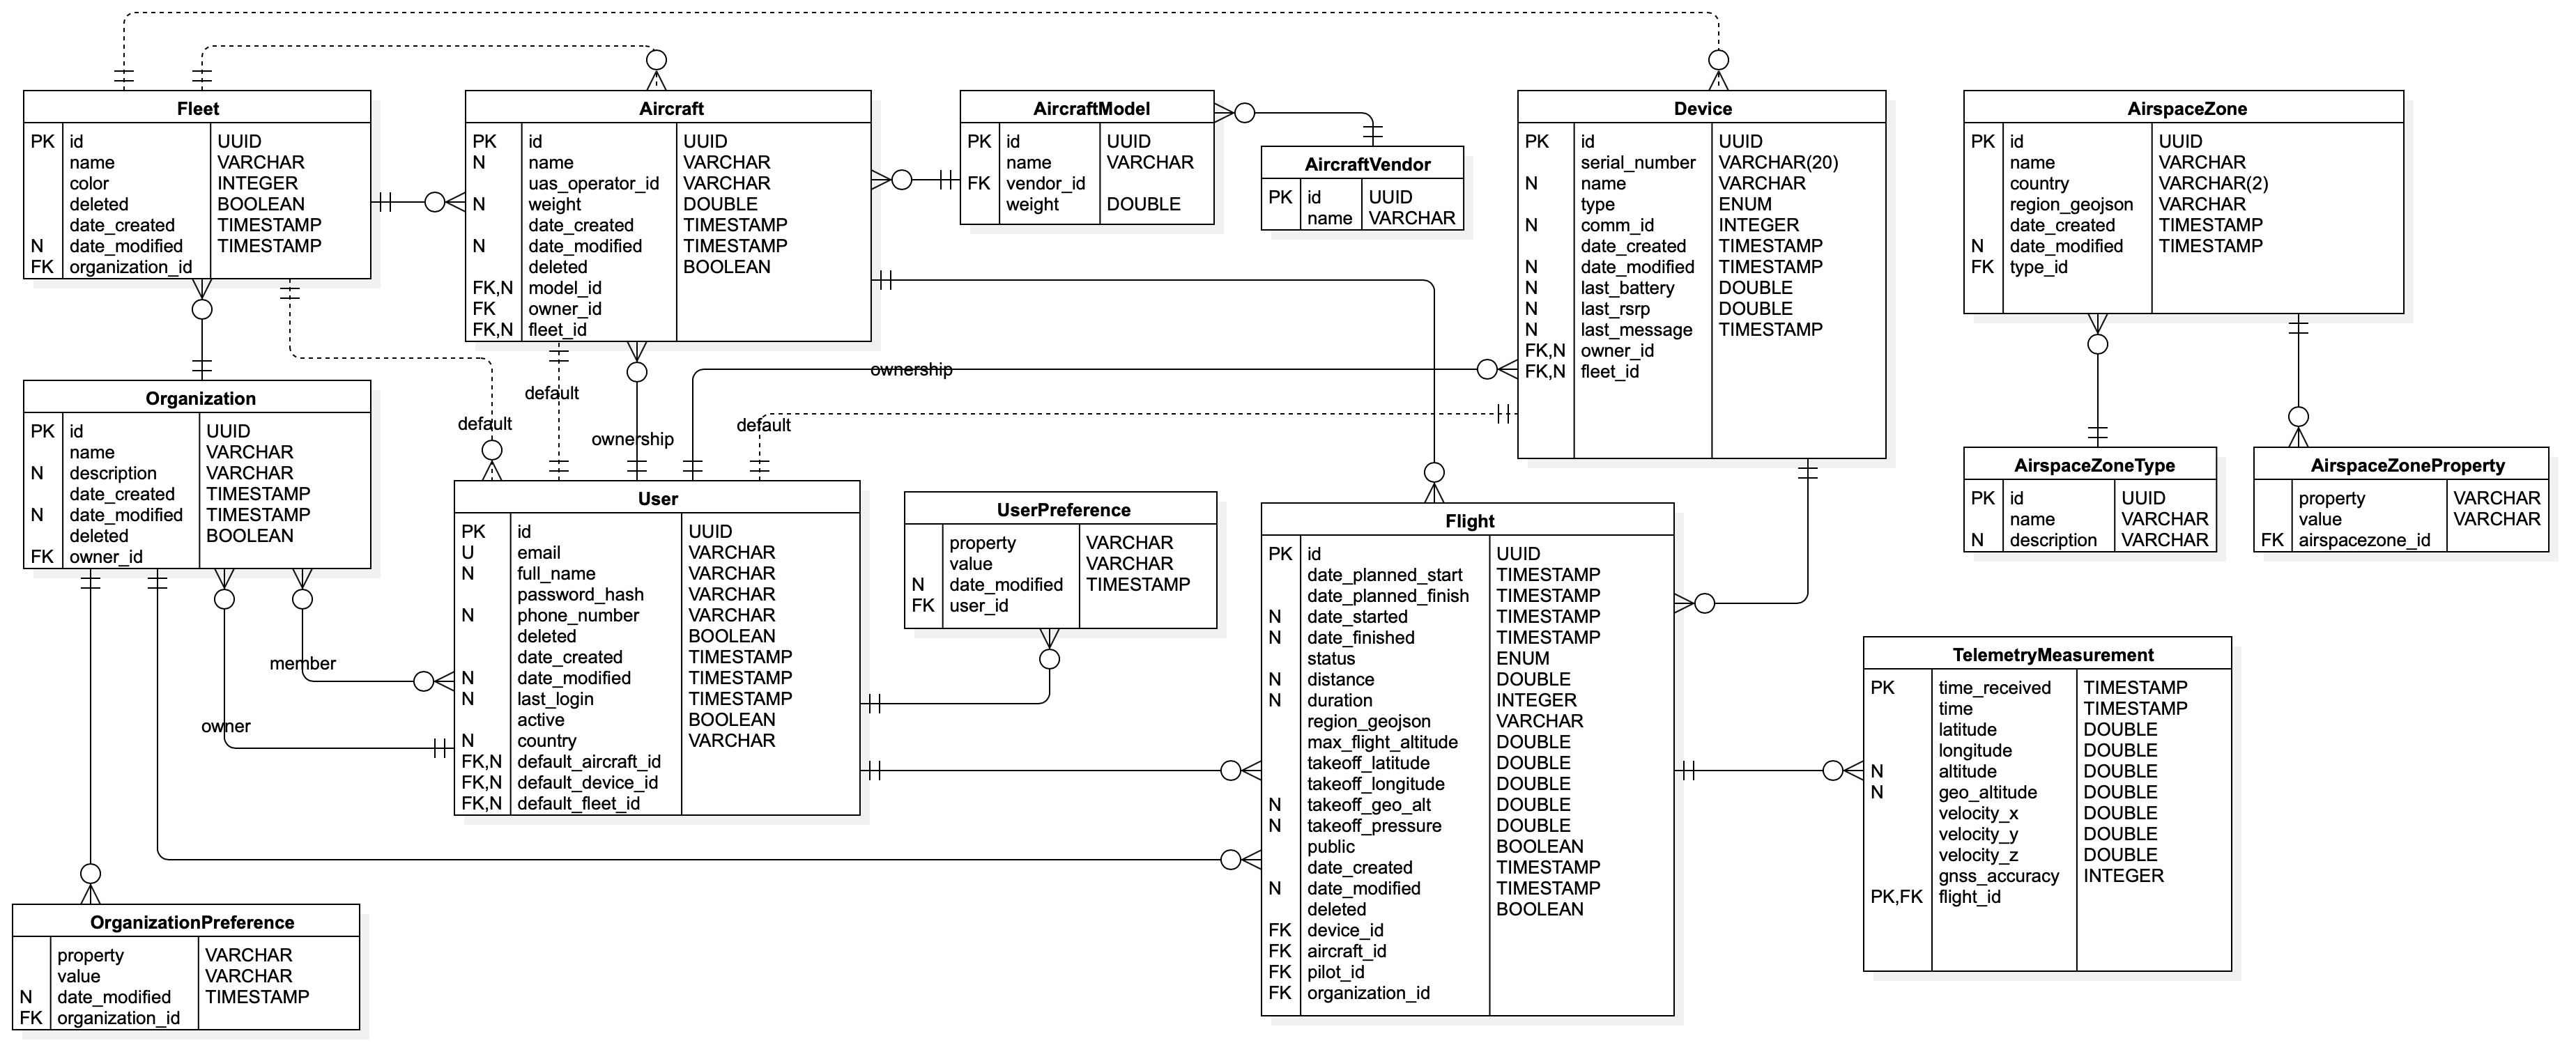
\includegraphics[scale=0.31, angle=90]{assets/erd_diagram.png}
    \caption{ERD Diagram of data model\cite{dataModel}}
    \label{fig:erd-diagram}
\end{figure}

\subsection{Live Service database model}\label{subsec:live-service-database-model}
In additional, during the development we had found out the current backend is not sufficient for our needs, so we decided to divide the backend model into backend one and Live Service model.
Because there are only live real time temporary data, so we deployed a Redis database.

"Redis is an open source (BSD licensed), in-memory data structure store, used as a database, cache and message broker.
It supports data structures such as strings, hashes, lists, sets, sorted sets with range queries, bitmaps, hyperloglogs, geospatial indexes with radius queries and streams.
Redis has built-in replication, Lua scripting, LRU eviction, transactions and different levels of on-disk persistence, and provides high availability via Redis Sentinel and automatic partitioning with Redis Cluster."\cite{redis}
It means that the Redis is a real-time storage that persists data only for very short time.
That is the reason, why it is suitable for this purpose.

The Live Service database model consists of \textbf{Device} and \textbf{Telemetry} entity.

